\chapter{Interface}

In this chapter we will be working on the background and the sound in the game. Again, a test app should be created to test these classes.

\section{Background}
The class for the background is kept simple. We never change anything in the background, so a \eeFunc{create} and \eeFunc{} method are all you need. We will never need more than one instance of this class. That's why we will create an instance of this class right below its declaration.

The playing field will look like figure \ref{fig:tetris_background}. Use it as a reference during the construction of this class.

\begin{figure}[ht]
\centering
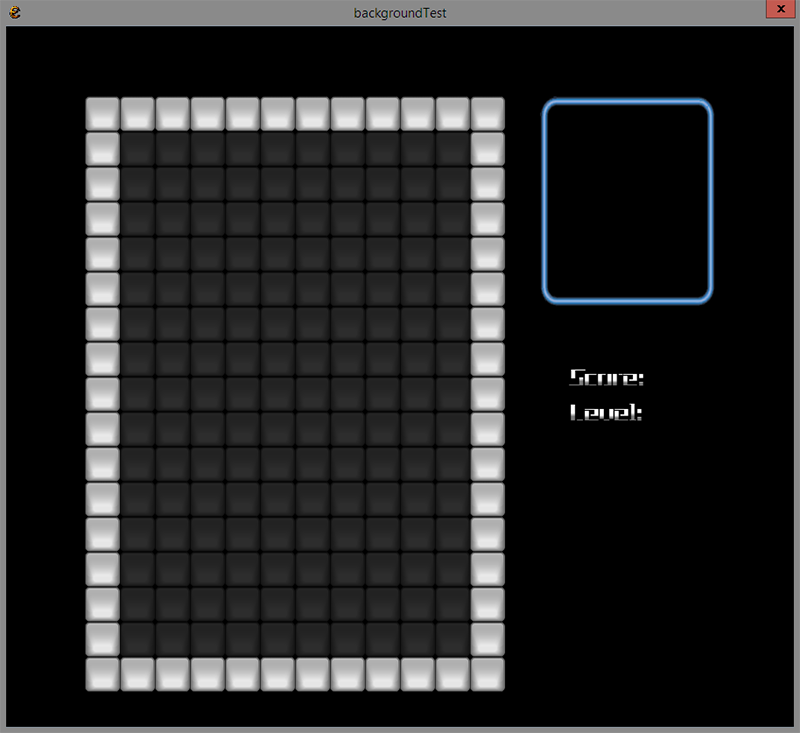
\includegraphics[width=0.6\linewidth]{images/tetris_background.png}
\caption[]{The Tetris background}
\label{fig:tetris_background}
\end{figure}

To draw the playing field we use squares. This also could be a picture, but the squares are easy to construct and rather fitting for this game. In addition, you need a \eeClass{Rectangle} to display an image on the position where the next block appears. Finally, we need to know the position where the score and the level should be drawn.

\begin{code}
class background
{
   Mems<square> squares;
   Rect blockRect;
   Vec2 scorePos;
   Vec2 levelPos;
   
   void create()
   {
   }
   
   void draw()
   {
   }
}

background Background;
\end{code}

In your test app, you can already use the two methods of this class. In addition, add the following line to the \eeFunc{InitPre} function:

\begin{code}
D.mode(WINDOW_WIDTH, WINDOW_HEIGHT);
\end{code}

This rule ensures that the application window is sized according to our constants. In the previous test program it was not necessary to do so, but with the background we want to see the final result.

\subsection{Playing Field}

As you know, the playing field is a grid. Because we will put a `wall' around the playing field, we don't start at position 0 but rather at position -1 to add squares. The squares in the field itself will have the type \eeFunc{BT\_BACKGROUND}. The walls have the type \eeFunc{BT\_WALL}. Because of this they will be put on the screen in a different color.

The code to add the necessary squares is shown below. Actually it is not that difficult to understand, but you might have no idea how to start on this. Read this code to gain a full understanding on how this works. Then add it to the \eeFunc{create} method.

\begin{code}
for(int x = -1; x <= SQUARES_PER_ROW; x++)
{
  for(int y = -1; y <= ROWS; y++)
  {
    if(x == -1 || y == -1 || x == SQUARES_PER_ROW || y == ROWS)
    {
      squares.New().create(VecI2(x, y), BT_WALL);
    } else {
      squares.New().create(VecI2(x, y), BT_BACKGROUND);
    }
  }
}
\end{code}

In the draw method you start with a black background. Next you show all the elements of the `squares' container. Test your app and verify the result.

\subsection{Next Block}
At the position where the next block appears, we draw an image. We've already made a constant for this position: \eeFunc{WAITPOS}. But that is a position in the grid. So we should always multiply this position with the size of a square (the constant \eeFunc{SQUARE\_SIZE}). Moreover, we should start at the position of the playing field, which is the constant \eeFunc{GAMEAREA}.

We can therefore calculate the following position:

\begin{code}
Vec2 blockPos = GAMEAREA + (WAITPOS * SQUARE_SIZE);
\end{code}

But as you know a rectangle requires a minimum and a maximum position. To calculate the minimum, you subtract two squares of the detected position. It would be logical add extra two squares for the maximum position. But later on you will see that this looks less good. This is no problem. You can change this code whenever you like. The last line uses the two new values ​​in order to set the actual rectangle.

\begin{code}
Vec2 min = blockPos - (2 * SQUARE_SIZE);
Vec2 max = blockPos + (2 * SQUARE_SIZE);
blockRect.set(min, max);
\end{code}

Now add code to the \eeFunc{draw} method to draw the picture `Tetris\_next\_bg' using the rectangle you've just created.

\subsection{Text}
You still need two more positions: \eeFunc{scorePos} and \eeFunc{levelPos}. For the position of the score, blockPos will be used as a starting point. Subtract \eeFunc{SQUARE\_SIZE} four times of the vertical value. Now you need the position to draw the level. Start from the score position, and subtract another square.

Once you've done that, you are ready to draw the score on the screen. Right now, it will suffice to show a random text. The real score will be added later. Besides, a special font is supplied with this template project. You will find it in gui $\Rightarrow$ tetrisFont $\Rightarrow$ tetris Style. If you do not know how to customize the look of text, you can review Chapter \ref{chapter:tekstopmaak}.

Test your application when you're done.

\section{Sound}
The next class is \eeClass{soundManager}. This one is pretty simple and you surely can write it yourself. There are no create methods required, only methods which play a particular sound. You will write these methods:

\begin{enumerate}
  \item startMusic: Start the soundtrack in a loop.
	\item blip: play the `blip' sound.
	\item score: play the `rowdone' sound.
	\item win: play the 'won' sound.
	\item list: play the `lost' sound.
	\item rotate: play the 'rotate' sound.
	\item moveDown: playing the `down' sound.
\end{enumerate}

This class also needs only one instance, so you should create the a \eeClass{SoundManager} below the class definition. Once done, you can create a little test in which you press keys to play a certain sound. Ensure that all sounds equally loud. If necessary, you can adjust the volume of certain sounds.
